\section{Nuclear Star Clusters and their Host Galaxies}\label{sec:hosts}
%key points: \\
%- early studies indicated that nucleation fraction is dE,N galaxies in Virgo is a function of luminosity
%- this was later (Cote et al. 2006) shown to be mostly a bias caused by the observational limitations

\begin{figure}
    \centering
%    \plottwo{./Figures/mnuc_mgal.pdf}{./Figures/frac_mnsc_mgal.pdf}
    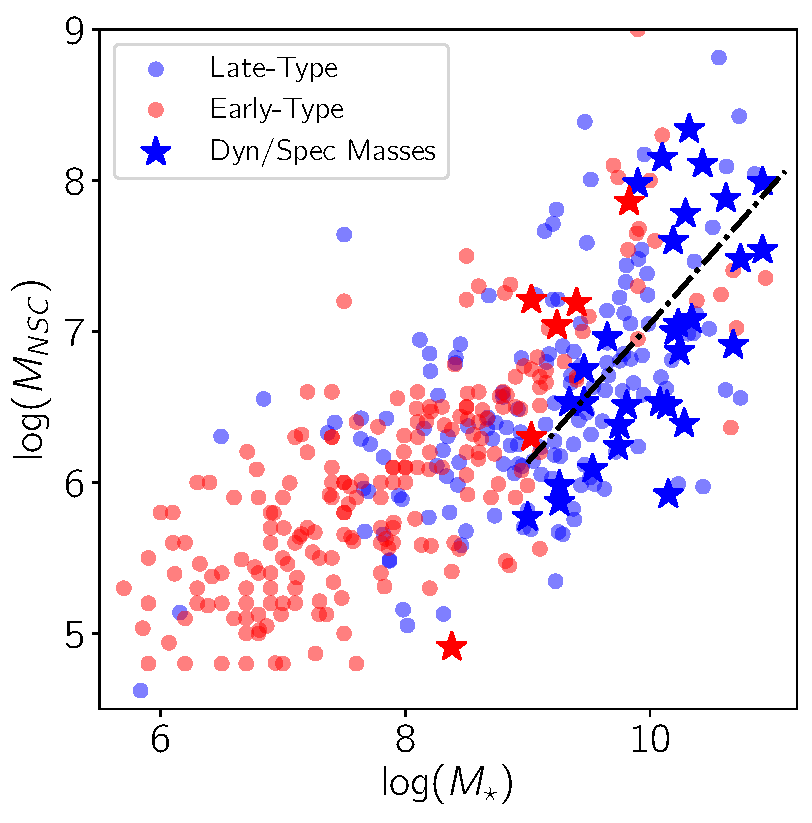
\includegraphics[width=0.45\textwidth]{./Figures/mnuc_mgal.pdf}
    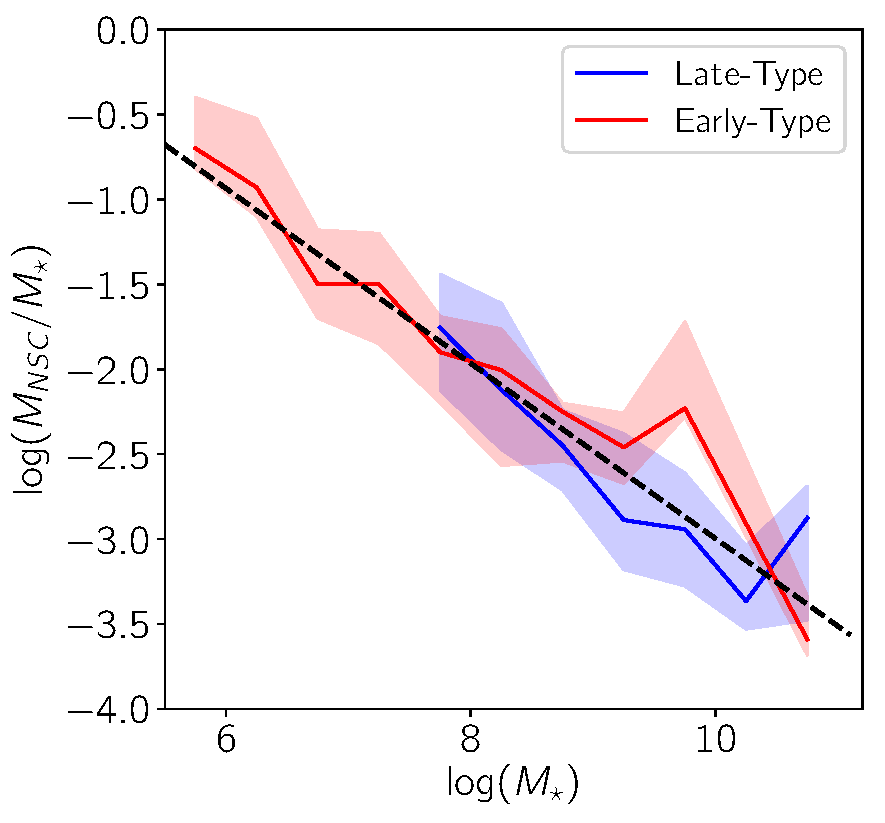
\includegraphics[width=0.48\textwidth]{./Figures/frac_mnsc_mgal.pdf}
    \caption{The masses of nuclear star clusters correlate with galaxy masses, but higher mass galaxies have a lower fraction of their mass in their NSC.  {\em Left --} Galaxy and NSC masses for galaxies in which both quantities are available.  The compilation of dynamical and spectroscopically modeled NSC masses from \citet{erwin12} is shown with stars, while all other masses are derived from colors using stellar population models with a Chabrier or Kroupa IMF \citep{georgiev16,spengler17,ordenes-briceno18,sanchez-janssen19}.  Galaxies have been divided by their Hubble types into early and late-types. {\em Right --}  The mass fraction of galaxies in NSCs as a function of galaxy mass, using the data from the left panel.  The line indicates the median galaxy within each mass bin, while shaded regions show the 25th and 75th percentiles of the distribution. }
    \label{fig:mass_scaling}
\end{figure}

In this section we consider how NSCs are related to the host galaxies they live in.  First we discuss the overall scaling of NSC mass with galaxy properties.



\subsection{Scaling Relations of NSCs}\label{subsec:scaling}

The most straightforward quantities to compare between galaxies and NSCs are their luminosities and stellar masses, and there is a quite substantial body of literature that has examined these correlations.  The NSC luminosity was first compared to the host galaxy/bulge luminosity for small samples of galaxies by \citet{balcells03} and \citet{graham03}, and inspired by the BH scaling relations, subsequent papers examined a wide range of NSC--galaxy scaling relations in both luminosity and mass \citep{ferrarese06,wehner06,rossa06,balcells07,seth08b,erwin12,scott13,denbrok14,sanchez-janssen19}.  While it was at one point claimed that the NSC and BH scaling relations may be comparable \citep{ferrarese06,wehner06}, it is now clear that the NSC scaling relations are distinct from the BH scaling relations \citep{erwin12,scott13}.  We discuss this issue further in Section~\ref{sec:nsc-mbh}.  
%\citep{balcells03,ferrarese06,wehner06,rossa06,seth08,}

In the left panel of Figure~\ref{fig:mass_scaling} we show a compilation of NSC and galaxy masses based on the same sample shown in Fig.~\ref{fig:demographics}, with the addition of objects where the NSC masses have been measured using stellar population model fits or dynamical estimates  \citep[plotted as stars;][]{erwin12, nguyen18}.  
The best-fit log-linear relation to the full sample of 407 NSC and galaxy mass estimates is:
\begin{equation}
    {\rm log}\,M_{NSC} = 0.48\,{\rm log}\, \left( \frac{M_\star}{10^9 {\rm M}_\odot} \right) + 6.51
\end{equation}
Bootstrapping errors on both parameters of this fit are $\sim$0.04 dex, while the scatter around the fit is $\sim$0.6 dex.  While the errors on estimate M/L ratios for the individual measurements are large and heterogeneous, they should be below $\sim$0.3 dex \citep{roediger15}, and thus the scatter primarily reflects intrinsic scatter.  

This NSC--stellar mass scaling relation is consistent with 
%a large number of 
previous results \citep{balcells03,scott13,denbrok14,sanchez-janssen19}, and suggests that roughly $M_{NSC} \propto M_\star^{1/2}$.  This sub-linear trend means that NSCs in lower-mass galaxies typically make up a higher fraction of the galaxy mass than in higher-mass galaxies.  At 10$^9$~M$_
\odot$, this mass is about 0.3\% of the total galaxy mass, in agreement with the findings from \citet{cote06}.  The NSC-galaxy mass fraction is shown in the right panel of Figure~\ref{fig:mass_scaling}, which shows clearly that the mass scaling is very similar for both early- and late-type galaxies.  We will discuss this result in context of formation models in Section~\ref{sec:formation}.   

Both panels indicate that the high mass end of NSCs may behave somewhat differently, with a possible steepening of the NSC mass scaling slope.  For early types, this steepening has previously been noted by \citet{denbrok14} and by \citet{sanchez-janssen19}. At the same time, \citet{scott13} exclude these more massive objects as apparent nuclear stellar disks with larger effective radii rather than NSCs.  Given our inclusive defintion of NSCs these objects remain in our sample, but we nonetheless maintain a shallow slope even at higher masses including all objects.  If we restrict ourselves to the smaller subsample of objects with more accurate NSC mass measurements (shown in stars) we do find a steeper slope, which in this case is driven  primarily by massive NSCs in late-type galaxies.  More specifically, fitting just these galaxies, we get a nearly linear relationship:
\begin{equation}
    {\rm log}\,M_{NSC} = 0.92\,{\rm log}\, \left( \frac{M_\star}{10^9 {\rm M}_\odot} \right) + 6.13
\end{equation}
with bootstrapping uncertainties of $\sim$0.18 dex on both quantities.  This line is shown as a dot-dashed line in the right panel.  Hints of this linear mass scaling relationship are also seen in the full sample of galaxies in the right panel, where the early type galaxies have a bump above the best-fit relation above $10^9$~M$_\odot$, and the late-type galaxies show a modest flattening at the highest mass end.  We note that the lower mass fraction in the highest early-type bin in the right panel is due to our inclusion of galaxies from the \citet{lauer05} sample, which have not been included in previous scaling relation work \citep[i.e.][]{scott13,sanchez-janssen19}.  Surprisingly, these objects seem to follow the trend found for early-types at lower masses rather than follow the upturn found by \citet{sanchez-janssen19}.  

Probably still need to add something on M-$\sigma$ and other NSC relations?

\subsection{Other correlations between NSCs and their hosts}

 We have already touched on several links between galaxies and their hosts apart from their scaling relationships, which we summarize here.  First, in Section~\ref{sec:demographics} we showed that there is a clear dependence of the nucleation fraction of galaxies based on their stellar mass, and also (at least for lower mass early type galaxies) an environmental dependence.  At low masses, this dependence seems to be independent of galaxy type, rising steadily from lower masses to stellar masses $\sim$10$^9$~M$_\odot$.  At these same masses, \citet{sanchez-janssen19} find that the nucleation fraction is environmentally dependent, with massive galaxy clusters having more nucleated galaxies than less massive galaxy clusters and groups.  

The stellar populations of NSCs (Section~\ref{subsec:stelpop}) also seem to be correlated with those of their host galaxy in several interesting ways.  Spectroscopic studies suggest a correlation between galaxy and NSC star formation histories \citep[e.g.][]{kacharov18}.  This correlation breaks down in several interesting ways in early-type galaxies.  The NSC spectroscopic metallicities change significantly with galaxy mass (Fig.~\ref{fig:mass_metallicity}), while the relative colors of the NSC and galaxy also change with galaxy mass \citep{turner12,sanchez-janssen19}; they are typically bluer than their host galaxy at low masses (indicating lower metallicities or younger ages), but become redder for higher mass systems. We will discuss the formation implications of these results further in the next section.

%As mentioned earlier, the main diagnostic to indicate the presence of a NSC is a distinct upturn in the surface brightness profile inside the central few pc, i.e. a `light excess' above the inward extrapolation of the host galaxy disk/bulge (see Fig. 1 for examples). It should be noted, however, that this is not always a binary `yes or no' criterion, in the sense that there appears to be a continuous range for the amount of light excess which in early-type galaxies smoothly varies with host galaxy magnitude \citep{cote07}. Fainter galaxies have the largest excess, which becomes smaller and smaller for more and more massive hosts, such that the most massive ellipticals even show a central {\em light deficit}. 
